% !TeX spellcheck = nb_NO
\documentclass[english,a4paper,11pt]{article}
\usepackage{setspace}
\usepackage{listings}
\usepackage[dvipsnames]{xcolor}
\usepackage{babel}
\usepackage{bookman}
\usepackage[utf8]{inputenx}
\usepackage[T1]{fontenc}
\usepackage{xspace}
\usepackage{lastpage}
\usepackage{fancyhdr}
\usepackage{tabularx}
\usepackage{tikz}
\usepackage[normalem]{ulem}

\usepackage{varioref}
\usepackage{url}
\usepackage{moreverb}
\usepackage{ifthen}
\usepackage{amsmath}
\usepackage{siunitx}
%\usepackage{esint}
%\usepackage{mathdesign}
\usepackage{color}
\usepackage[version=4]{mhchem}
\usepackage[a4paper,left=15mm,right=30mm,top=25mm,bottom=25mm]{geometry}

\definecolor{codebg}{HTML}{fff5eb}

% set the default code style
\lstset{
	numberstyle=\tiny,
	frame=tb,
    tabsize=4,
    showstringspaces=false,
    numbers=left,
    commentstyle=\color{green},
    keywordstyle=\color{blue},
	stringstyle=\color{red},
	backgroundcolor=\color{codebg},
	basicstyle=\ttfamily\bfseries\color{black}
}

\usetikzlibrary{trees,arrows,arrows.meta,intersections,calc,backgrounds,positioning,decorations}
\setlength{\parskip}{1ex plus 4pt minus 2pt}
\setlength{\marginparwidth}{18mm}
\newcommand{\pagebottomtext}{
	\pagestyle{fancy}
	\renewcommand{\headrulewidth}{0pt}
	\fancyhead{}
	\cfoot{\rule{8em}{1pt}\\
		Page \thepage\ of \pageref{LastPage}}
}

\definecolor{verbalcolor}{rgb}{0.5,0.0,1.0}
\newcommand{\verbal}[1]{\texttt{\ttfamily\guillemotleft\textcolor{verbalcolor}{#1}\guillemotright}}
\newcommand{\marked}[1]{\textbf{#1}\xspace}

\definecolor{todo}{rgb}{0.5,0.0,0.0}
\definecolor{markup}{rgb}{0.0,0.0,1.0}
\newcommand{\todo}[1]{\par\textcolor{todo}{\bfseries TODO: #1}\par}

\newcommand{\entity}[1]{\texttt{\textcolor{markup}{\&#1;}}\xspace}
\newcommand{\numentity}[1]{\texttt{\textcolor{markup}{\&\#{}#1;}}\xspace}

\newenvironment{codeblock}{\begin{quote}\color{markup}}{\end{quote}}

\newcommand{\element}[1]{\textcolor{markup}{\texttt{#1}}\xspace}

\newcommand{\markup}[1]{\textcolor{markup}{\texttt{#1}}\xspace}

\newcommand{\listofdemands}[1]{
	\par\bigskip
	\textbf{Please note the following:}
	\begin{itemize}
		#1
	\end{itemize}
}

\newenvironment{examples}{
	\par\bigskip
	\textbf{Examples:}\par\medskip
	}{
	\par
}

\newcommand{\codesnippet}[1]{%
	% #1: kodesnippet
	\textcolor{blue}{\texttt{#1}}%
}


\title{Requirements for MathML markup\\ in EPUB files}
\author{NLB, MTM, SPSM, Celia, Nota, HBS, Dedicon}

\begin{document}
	\pagebottomtext
	\thispagestyle{empty}
	\raggedright
	
	\maketitle
	\thispagestyle{empty}
	\vfill
	\begin{quote} {
		\bigskip
		\emph{Version history:}\\
		\textbullet\quad20181220 / 1.0: First version\\
		\textbullet\quad20190130 / 1.1: Many new topics added, and small edits.\\
		\textbullet\quad20190926 / 1.2: Minor changes and additions.\\
		\textbullet\quad20191204 / 2.0: Conclusion of testing and linear math.\\
        \textbullet\quad20200206 / 2.1: Minor changes and additions.\\
        \textbullet\quad20200527 / 2.2: Clarifications.\\
        \textbullet\quad20200831 / 2.3: Update for language and more structure to chemistry markup.\\
        \textbullet\quad20200917 / 2.4: Added programming markup.\\
        \textbullet\quad20200928 / 2.5: Clarifications and updated code appearance.\\
        \textbullet\quad20220202 / 2.6: (current version) Clarifications for xml:lang, tables and identifiers/text.\\
        \bigskip
	}
	\end{quote}
	\vfill
	\pagebreak
	\tableofcontents
	\vfill
	\pagebreak

\section{The purpose of MathML in NLB's EPUB files}

NLB will use MathML in the EPUB files to present mathematical expressions in a variety of ways in the distributed versions of the content:
\begin{itemize}
	\item In a talking book version, we may synchronize a narrated version of the expression to the standard mathematical notation, the latter being generated automatically from MathML by the browser displaying the math as well as the text content of the talking book.

	\item In an e-book version we may present a MathML expression in the normal way; as a standard mathematical expression, using standard mathematical notation. In addition, we may present an automatically generated  textual representation of the mathematical expression, as an alternative or a supplement to those who prefer to use local synthetic speech or refreshable Braille to digest the content.
	
	\item In a TTS based talking book version, we may automatically generate a string that represents a verbal interpretation of the MathML. This string can then be used as a basis for TTS generation of an audio segment that represents the mathematical expression.

	\item The MathML version of a mathematical expression can be used as a basis for AsciiMath and printed Braille. Once again, the MathML may be converted to either AsciiMath or text, and this version may then be refined and converted to Braille.
\end{itemize}
Except for the first bullet point, which relies on the math knowledge of a  human narrator, production of the distributed version involve some kind of automatic transformation of the MathML markup into some other kind of textual representation, typically a pure text string containing a verbal representation of the math in question. 

\section{The fundamental requirements}

\begin{itemize}
	\item All mathematical expressions --~both inline and block~-- shall be marked up, along with the general EPUB markup, using \emph{MathML Presentation Markup}, as specified in ''Mathematical Markup Language (MathML) Version 3.0 2nd Edition''\footnote{See~\url{https://www.w3.org/TR/MathML3/}}.
	\item The language of the generated text is reliant on which \emph{xml:lang}-attribute is set. Thus there must exist an ancestor of the expression with the \emph{xml:lang}-attribute, for example: \element{<html xml:lang="en">} or \element{<html xml:lang="en"><body><div xml:lang="no"><m:math>...</m:math></div></body></html>}. A math element itself cannot contain a \element{xml:lang} attribute.
	\item Whenever applicable, the requirements in this document must be respected.
	
	\textbf{For mathematical expressions that are not covered in this document, the personnel involved in the markup process is encouraged to do MathML markup based on a good understanding of mathematics, combined with a solid knowledge of the set of MathML elements and attributes.}

	\item Unless MathML markup of a certain type of mathematical expression is specified in this document, the markup should be based on a good understanding of mathematics, combined with a solid knowledge of the set of MathML elements and attributes.
	\item Use the numeric XML annotation of an entity, for example: instead of \entity{ApplyFunction} or \entity{af}, use \entity{\#8289}, or it's unicode representation.
	\item All MathML markup must be annotated with an AsciiMath expression that represents the mathematical expression printed in the book. Thus, the complete markup of any given mathematical expression must be coded according to the following scheme:

\begin{lstlisting}[language=HTML, caption={Default MathML markup}]
<m:math xmlns:m="http://www.w3.org/1998/Math/MathML"
	alttext="[AsciiMath markup]" 
	altimg="[Image path]" 
	display="[block|inline]">
	<m:semantics>
		<m:mrow>
			[MathML markup]
		</m:mrow>
	</m:semantics>
</m:math>
\end{lstlisting}

	The \markup{[MathML markup]} is, obviously, the MathML markup that represents the mathematical expression in question, and \markup{[AsciiMath markup]} is the AciiMath version of the same expression.

Observe that the MathML markup will always be a child of an \element{mrow} element, which again is a child of an \element{semantics} element, which again is a child of an \element{math} element, which constitute the frame around the complete MathML markup.

\bigskip
Please consult \url{https://www.w3.org/TR/MathML3/chapter5.html#mixing.semantic.annotations} for further information about annotation of MathML markup.
\end{itemize}

\subsection{The display attribute}

The \markup{display} attribute must be included and used correctly on the \element{<math>} element. The value of the \markup{display} attribute shall always be either \markup{block} or \markup{inline}, depending on the placement of the expression in the printed book.

\bigskip
\textbf{From the MathML 3 specification:}

specifies whether the enclosed MathML expression should be rendered as a separate vertical block (in display style) or inline, aligned with adjacent text.

\url{https://www.w3.org/TR/MathML3/chapter2.html#interf.toplevel}

\bigskip
\textbf{From the description on mozilla.org:}

This enumerated attribute specifies how the enclosed MathML markup should be rendered. It can have one of the following values:

\textit{block}, which means that this element will be displayed outside the current span of text, as a block that can be positioned anywhere without changing the meaning of the text;

\textit{inline}, which means that this element will be displayed inside the current span of text, and cannot be moved out of it without changing the meaning of that text.

\url{https://developer.mozilla.org/en-US/docs/Web/MathML/Element/math#attr-display}

\bigskip
\textbf{It should be possible to implement this in practice using the following rules:}
\begin{itemize}
    \item If the \element{<math>} element has a sibling node which is either a non-empty text node (note that text nodes consisting only of whitespace are considered "empty"), or one of the following inline elements, then the \markup{display} attribute should be set to inline: \element{<a>}, \element{<abbr>}, \element{<bdo>}, \element{<br>}, \element{<code>}, \element{<dfn>}, \element{<em>}, \element{<img>}, \element{<kbd>}, \element{<q>}, \element{<samp>}, \element{<span>}, \element{<strong>}, \element{<sub>}, \element{<sup>}.
    \item The \element{<math>} element must not be the only node in an inline context.
    
    So for instance, while \markup{<p><math display="inline">…</math></p>} is technically valid, it should rather be written as \markup{<math display="block">…</math>}. 
    
    But if there are non-empty text nodes or inline elements in the same context, then \markup{display="inline"} should still be used: \markup{<p>text text <math display="inline">…</math> <span>more text</span></p>} is correct.
    \item \element{<math>} elements that are not in an inline context, should use \markup{display="block"}.
\end{itemize}

See also: \url{https://developer.mozilla.org/en-US/docs/Web/HTML/Inline_elements}

\bigskip

Please note that, in all of the examples to follow, the markup discussed is the one represented by the \markup{[MathML markup]} part. The outer \element{math}, \element{semantics} and \element{mrow} framework is omitted, to put focus on the matter in question. These elements are of course always required as a container for each of the mathematical expressions in the EPUB file.

\begin{center}
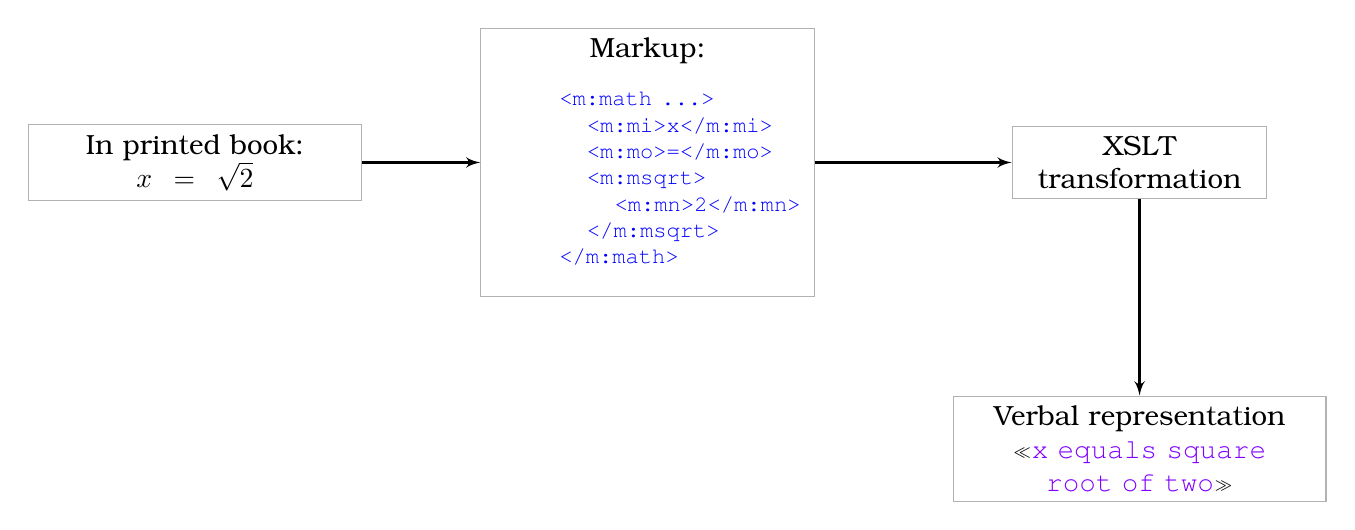
\begin{tikzpicture}
\node[text width=40mm,align=center,draw=black!30] (matte) {In printed book:\\$x =\sqrt{2}$};

\node[text width=40mm,align=center,draw=black!30,right=15mm of matte] (MathML) {Markup:
\begin{codeblock}
\footnotesize
\begin{verbatimtab}[3]
<m:math ...>
	<m:mi>x</m:mi>
	<m:mo>=</m:mo>
	<m:msqrt>
		<m:mn>2</m:mn>
	</m:msqrt>
</m:math>
\end{verbatimtab}
\end{codeblock}
};

\node[text width=30mm,align=center,draw=black!30,right=25mm of MathML] (xslt) {XSLT \mbox{transformation}};
\node[text width=45mm,align=center,draw=black!30,below=25mm of xslt] (tale) {Verbal \mbox{representation}\\\verbal{x equals square root of two}};

\draw[-latex',thick] (matte) -- (MathML);
\draw[-latex',thick] (MathML) -- (xslt);
\draw[-latex',thick] (xslt) -- (tale);
\end{tikzpicture}
\end{center}
The quality of the generated text string relies heavily on the quality of the MathML markup, and care must be taken to create MathML markup that~\ldots
\begin{itemize}
	\item \ldots correctly represents the printed mathematical expressions;
	\item \ldots is compliant with the W3C recommendations for use of MathML markup;
	\item \ldots respects the NLB specific requirements stated in this document;
	\item \ldots ensures that the mathematical information that can be detected from the markup, is as unambiguous as possible.
\end{itemize}
The last point is very important, as the interpretation of a mathematical expression often relies on the context  the expression is placed in, and also on the interpreter's (e.g. the student's) understanding of that context.

As an example, we can investigate the following expression:
\begin{equation}
a (t + \varphi)
\end{equation}
One interpretation of this expression is that it represents a variable, $a$, that is to be multiplied by the sum of two other variables, $t + \varphi$.
 
A completely different interpretation is that the expression represents a function, $a$, with one argument, namely the sum of $t$ and $\varphi$.

It is extremely important that the interpretation is clearly indicated in the MathML markup. If the expression represents a multiplication operation, this should be clarified by use of the MathML operator
\verb|<m:mo>&#8290;</m:mo>|. And similar, the representation of a function must be clarified by using
\verb|<m:mo>&#8289;</m:mo>|.


So, even though this:
\begin{lstlisting}[language=HTML]
<m:math xmlns="http://www.w3.org/1998/Math/MathML" display="block">
	<m:mi>a</m:mi>
	<m:mo>(</m:mo>
	<m:mi>t</m:mi>
	<m:mo>+</m:mo>
	<m:mi>&#966;</m:mi>
	<m:mo>)</m:mo>
</m:math>
\end{lstlisting}
in many cases would be perfectly good markup of the expression above, NLB require the markup to be either
\begin{lstlisting}[language=HTML]
<m:math xmlns="http://www.w3.org/1998/Math/MathML" display="block">
	<m:mi>a</m:mi>
	<m:mo>&#8290;</m:mo>
	<m:mfenced open="(" close=")">
		<m:mrow>
			<m:mi>t</m:mi>
			<m:mo>+</m:mo>
			<m:mi>&#966;</m:mi>
		</m:mrow>
	</m:mfenced>
</m:math>
\end{lstlisting}
for the ''multiplication interpretation'', or
\begin{lstlisting}[language=HTML]
<m:math xmlns="http://www.w3.org/1998/Math/MathML" display="block">
	<m:mi>a</m:mi>
	<m:mo>&#8289;</m:mo>
	<m:mfenced open="(" close=")">
		<m:mrow>
			<m:mi>t</m:mi>
			<m:mo>+</m:mo>
			<m:mi>&#966;</m:mi>
		</m:mrow>
	</m:mfenced>
</m:math>
\end{lstlisting}
for the ''function interpretation''. Note that the only difference is the choice of entity in line~3.

It should be quite clear by now that, to ensure the expected quality of the MathML markup, personnel with solid mathematical skills, as well as the ability to focus on important markup details, must be assigned to this kind of work.


If the expression above stands completely alone, it is not possible to decide the correct representation. However, if there is an overlaying context, perhaps if the expression above is part of a larger mathematical expression, the representation should be clear enough.

This equation
\begin{equation}
a (t + \varphi) = a \cdot t + a \cdot \varphi
\end{equation}
clearly indicates that we are talking about multiplication, while
\begin{equation}
a (t + \varphi) = \frac{\partial^2 x(t + \varphi)}{\partial t^2}
\end{equation}
indicates that we are talking about functions, perhaps related to acceleration and position.

\bigskip

This document aims to specify the exact markup we want, when there seems to be different ways to use MathML to represent the mathematical expression. If you cannot find a description on a specific notation in this document, please refer to the Mathematical Markup Language (MathML) Version 3.0 2nd Edition of 10th of April, 2014 \url{https://www.w3.org/TR/MathML3/}. 

\bigskip

Note that this is a work in progress; the scope of mathematical topics to be covered will certainly be widened in the future. You should also expect changes in established requirements as we gain experience with the automatic transformation of MathML to alternative formats.

\vfill
\pagebreak

\section{Additional requirements and examples}

\subsection{Use of invisible operators}

If there is any risk of ambiguity, the following operators \textbf{must} be used as entities in the markup:

\begin{tabular}{llll}
\multicolumn{1}{c}{\textbf{Entity}}
		& \multicolumn{1}{c}{\textbf{Numeric}}
			& \multicolumn{1}{c}{\textbf{Comment}}\\
\entity{ApplyFunction} & \entity{\#8289} & Function application\\
\entity{InvisibleTimes} & \entity{\#8290} & Invisible multiplication\\
\entity{InvisibleComma} & \entity{\#8291} & Invisible separator\\
 & \entity{\#8292} & Invisible addition
\end{tabular}

This means that, even for expressions such as 
\begin{equation}
	(x+y) (x-y)
\end{equation}
or 
\begin{equation}
	2 \sin \alpha
\end{equation}
where it is quite clear from the context that multiplication is involved, we \emph{require} that these multiplications are added to the markup. Thus, expression 4 must be marked up as 

\begin{lstlisting}[language=HTML, caption={Invisible multiplication}]
<m:mfenced open="(" close=")">
	<m:mrow>
		<m:mi>x</m:mi>
		<m:mo>+</m:mo>
		<m:mi>y</m:mi>
	</m:mrow>
</m:mfenced>
<m:mo>&#8290;</m:mo>
<m:mfenced open="(" close=")">
	<m:mrow>
		<m:mi>x</m:mi>
		<m:mo>-</m:mo>
		<m:mi>y</m:mi>
	</m:mrow>
</m:mfenced>
\end{lstlisting}
while expression 5 must be represented with the following markup:
\begin{lstlisting}[language=HTML, caption={Function application and invisible multiplication}]
<m:mn>2</m:mn>
<m:mo>&#8290;</m:mo>
<m:mrow>
	<m:mi>sin</m:mi>
	<m:mo>&#8289;</m:mo>
	<m:mi>&#593;</m:mi>
</m:mrow>
\end{lstlisting}
Note the use of \entity{\#8290} in line~8 and line~2 respectively in these markup snippets.

Multiple examples of use of invisible operators are given in the following sections.

\subsection{Markup of less than, less than or equal, greater than and greater than or equal}

HTML entities would generally be able to be used for this, but to remove the risk of ambiguity, we will need them to be coded in the following manner:

\begin{tabular}{llll}
	\multicolumn{1}{c}{\textbf{Short}}
		& \multicolumn{1}{c}{\textbf{Numeric}}
			& \multicolumn{1}{c}{\textbf{Comment}}\\
	\entity{lt} & \entity{\#60} & Less than\\
	\entity{gt} & \entity{\#62} & Greater than\\
	& \entity{\#8804} & Less than or equal\\
    & \entity{\#8805} & Greater than or equal\\
\end{tabular}\\
\bigskip

\begin{lstlisting}[language=HTML, caption={$9 < 10$}]
<m:mrow> 
	<m:mn>9</m:mn>
	<m:mo>&#60;</m:mo>
	<m:mi>10</m:mi>
</m:mrow>
\end{lstlisting}
\bigskip
\begin{lstlisting}[language=HTML, caption={$10 > 9$}]
<m:mrow> 
	<m:mn>10</m:mn>
	<m:mo>&#62;</m:mo>
	<m:mi>9</m:mi>
</m:mrow>
\end{lstlisting}
\bigskip
\begin{lstlisting}[language=HTML, caption={$9 \leq 9$}]
<m:mrow> 
	<m:mn>9</m:mn>
	<m:mo>&#8804;</m:mo>
	<m:mi>9</m:mi>
</m:mrow>
\end{lstlisting}
\bigskip
\begin{lstlisting}[language=HTML, caption={$9 \geq 9$}]
<m:mrow> 
	<m:mn>9</m:mn>
	<m:mo>&#8805;</m:mo>
	<m:mi>9</m:mi>
</m:mrow>
\end{lstlisting}

\subsection{Markup of parenthesis}

Parenthesis shall not be marked up using \verb|<m:mo>(</m:mo>| and \verb|<m:mo>)</m:mo>|. Rather the MathML element \element{mfenced} must be used. 
The \element{mfenced} should contain attribute defining what type of parenthesis it, as follows: 
\begin{lstlisting}[language=HTML]
<m:mfenced open="(" close=")">
	<m:mi>x</m:mi>
</m:mfenced>
\end{lstlisting}
This is done to clarify what parenthesis we are dealing with.\\
\bigskip
There are other parentesis to be aware of:

\begin{lstlisting}[language=HTML, caption={Square bracket}]
<m:mfenced open="[" close="]">
	<m:mi>x</m:mi>
</m:mfenced>
\end{lstlisting}

\begin{lstlisting}[language=HTML, caption={Curly bracket}]
<m:mfenced open="{" close="}">
	<m:mi>x</m:mi>
</m:mfenced>
\end{lstlisting}

This is trivial when there is only one element inside the parenthesis, such as $g(x)$, which should be marked up as
\begin{lstlisting}[language=HTML]
<m:mrow>
	<m:mi>g</m:mi>
	<m:mo>&#8289;</m:mo>
	<m:mfenced open="(" close=")">
		<m:mi>x</m:mi>
	</m:mfenced>
</m:mrow>
\end{lstlisting}

However, when the content of the parenthesis consists of multiple parts, such as $3 \cdot (4 + 9)$, the content of the \element{mfenced} element must be placed inside an \element{mrow} element:
\begin{lstlisting}[language=HTML]
<m:mn>3</m:mn>
<m:mo>&#8901;</m:mo>
<m:mfenced open="(" close=")">
	<m:mrow>
		<m:mn>4</m:mn>
		<m:mo>+</m:mo>
		<m:mn>9</m:mn>
	</m:mrow>
</m:mfenced>
\end{lstlisting}
A more complex example, involving nested parenthesis, is
\begin{equation}
4 \cdot (x + x \cdot (x +a)) \cdot (x - x\cdot (x -b))
\end{equation}
The correct markup of this expression would be
\begin{lstlisting}[language=HTML]
<m:mn>4</m:mn>
<m:mo>&#8901;</m:mo>
<m:mfenced open="(" close=")">
	<m:mrow>
		<m:mi>x</m:mi>
		<m:mo>+</m:mo>
		<m:mi>x</m:mi>
		<m:mo>&#8901;</m:mo>
		<m:mfenced open="(" close=")">
			<m:mrow>
				<m:mi>x</m:mi>
				<m:mo>+</m:mo>
				<m:mi>a</m:mi>
			</m:mrow>
		</m:mfenced>
	</m:mrow>
</m:mfenced>
<m:mo>&#8901;</m:mo>
<m:mfenced open="(" close=")">
	<m:mrow>
        <m:mi>x</m:mi>
        <m:mo>-</m:mo>
        <m:mi>x</m:mi>
        <m:mo>&#8901;</m:mo>
        <m:mfenced open="(" close=")">
            <m:mrow>
                <m:mi>x</m:mi>
                <m:mo>-</m:mo>
                <m:mi>b</m:mi>
            </m:mrow>
        </m:mfenced>
	</m:mrow>
</m:mfenced>
\end{lstlisting}


\bigskip
Consult \url{https://www.w3.org/TR/MathML3/chapter3.html#presm.mfenced} for further information about use of the \element{mfenced} element.

\subsection{Markup of the absolute value}
The absolute value of a number, symbol or expression shall be done using the MathML element \element{mfenced} together with the \markup{open} and \markup{close} attributes. Both attributes must have the value \markup{|}.

The expression 
\begin{equation}|-2| = 2\end{equation}
must be marked up as
\begin{lstlisting}[language=HTML, caption={Absolute values}]
<m:mfenced open="|" close="|">
	<m:mrow>
		<m:mo>-</m:mo>
		<m:mn>2</m:mn>
	</m:mrow>
</m:mfenced>
<m:mo>=</m:mo>
<m:mn>2</m:mn>
\end{lstlisting}
while the more complex expression
\begin{equation}
\left|\cos \frac{x}{2}\right| =\sqrt{\frac{1 + \cos x}{2}}
\end{equation}
must be marked up as follows:
\begin{lstlisting}[language=HTML]
<m:mfenced open="|" close="|">
	<m:mrow>
		<m:mi>cos</m:mi>
		<m:mo>&#8289;</m:mo>
		<m:mfrac>
			<m:mi>x</m:mi>
			<m:mn>2</m:mn>
		</m:mfrac>
	</m:mrow>
</m:mfenced>
<m:mo>=</m:mo>
<m:msqrt>
	<m:mrow>
		<m:mfrac>
			<m:mrow>
				<m:mn>1</m:mn>
				<m:mo>+</m:mo>
				<m:mrow>
					<m:mi>cos</m:mi>
					<m:mo>&#8289;</m:mo>
					<m:mi>x</m:mi>
				</m:mrow>
			</m:mrow>
			<m:mn>2</m:mn>
		</m:mfrac>
	</m:mrow>
</m:msqrt>
\end{lstlisting}

\subsection{Markup of number of degrees}

How to mark up a number of degrees, such as such as $\ang{360}$ or $\ang{-273,15}\;\text{C}$, depends on whether the value is positive or negative.

For a positive number, the required markup is simple:
\begin{lstlisting}[language=HTML]
<m:mrow>
	<m:mn>[numeric value]</m:mn>
	<m:mi>&#176;</m:mi>
</m:mrow>
\end{lstlisting}

\listofdemands{
	\item The markup must be placed inside an \element{mrow} element. This \element{mrow} must contain exactly two children.
	\item The first child of the \element{mrow} element must be an \element{mn} element, containing the relevant value.
	\item The second child of the \element{mrow} must be an \element{mo} element, containing the degree symbol, represented by the numeric entity \numentity{176}.
}
Note also that the \element{msup} element must not be used, as the degree symbol by itself represents a raised ring.

\medskip
For a negative value, the required markup is a bit more complex:
\begin{lstlisting}[language=HTML]
<m:mrow>
	<m:mrow>
		<m:mo>-</m:mo>
		<m:mn>[numeric value]</m:mn>
	</m:mrow>
	<m:mi>&#176;</m:mi>
</m:mrow>
\end{lstlisting}

\listofdemands{
	\item Once again the markup must be placed inside an \element{mrow} element with exactly two children.
	\item However, this time the first child of the \element{mrow} element must be another \element{mrow} element:
	\begin{itemize}
		\item The first child of this \element{mrow} element must be an \element{mo} element containing the normal hyphen sign.
		\item The second child of this \element{mrow} element must be an \element{mn} element, containing the relevant absolute value.
	\end{itemize}
	\item The second child of the containing \element{mrow} element must be an \element{mo} element, containing the degree symbol, represented by the numeric entity \numentity{176}.
}

\medskip
This kind of markup is relevant both for  temperature and for angular measurements. But for angular measurements there is --~in addition to the normal 360 degree division of a circle~-- the \emph{gradian measure} where the circle is divided into 400~gon, so that $\ang{360} = 400^\text{g}$.

The required markup for this kind of angular measurement is either:
\begin{lstlisting}[language=HTML]
<m:msup>
	<m:mn>[numeric value]</m:mn>
	<m:mtext>g</m:mtext>
</m:msup>
\end{lstlisting}
or
\begin{lstlisting}[language=HTML]
<m:msup>
	<m:mrow>
		<m:mo>-</m:mo>
		<m:mn>[numeric value]</m:mn>
	</m:mrow>
	<m:mtext>g</m:mtext>
</m:msup>
\end{lstlisting}
depending on the value, as described above.

Note the use of the \element{msup} element this time, in order to raise the unit g.

\begin{examples}
The markup for the expression
\begin{equation}
\ang{0}\;\text{C} = \ang{32}\;\text{F} = 273\;\text{K}
\end{equation}	
is
\begin{lstlisting}[language=HTML]
<m:mrow>
	<m:mn>0</m:mn>
	<m:mi>&#176;</m:mi>
</m:mrow>
<m:mspace width="0.25em"/>
<m:mtext>C</m:mtext>
<m:mo>=</m:mo>
<m:mrow>
	<m:mn>32</m:mn>
	<m:mi>&#176;</m:mi>
</m:mrow>
<m:mspace width="0.25em"/>
<m:mtext>F</m:mtext>
<m:mo>=</m:mo>
<m:mn>273</m:mn>
<m:mspace width="0.25em"/>
<m:mtext>K</m:mtext>
\end{lstlisting}
Note the use of the \element{mspace} element to insert proper visual spacing between values and the relevant unit.

For clarity, one could use the following markup instead:
\begin{lstlisting}[language=HTML]
<m:mrow>
	<m:mrow>
		<m:mn>0</m:mn>
		<m:mi>&#176;</m:mi>
	</m:mrow>
	<m:mspace width="0.25em"/>
	<m:mtext>C</m:mtext>
</m:mrow>
<m:mo>=</m:mo>
<m:mrow>
	<m:mrow>
		<m:mn>32</m:mn>
		<m:mi>&#176;</m:mi>
	</m:mrow>
	<m:mspace width="0.25em"/>
	<m:mtext>F</m:mtext>
</m:mrow>
<m:mrow>
	<m:mo>=</m:mo>
	<m:mn>273</m:mn>
	<m:mspace width="0.25em"/>
	<m:mtext>K</m:mtext>
</m:mrow>
\end{lstlisting}
The only difference is the extra \element{mrow} elements that are used to group together the different parts of the expression.

The expression $T_0 = \ang{-273,15}\;\text{C}$ must be represented by the following markup:
\begin{lstlisting}[language=HTML]
<m:msub>
	<m:mi>T</m:mi>
	<m:mn>0</m:mn>
</m:msub>
<m:mo>=</m:mo>
<m:mrow>
	<m:mrow>
		<m:mo>-</m:mo>
		<m:mn>273,15</m:mn>
	</m:mrow>
	<m:mi>&#176;</m:mi>
</m:mrow>
<m:mspace width="0.25em"/>
<m:mtext>C</m:mtext>
\end{lstlisting}

As a final example, the expression \begin{equation}
\sin \ang{45} =\sin 50^\text{g}  = \sin\frac{\pi}{2}= \frac{1}{\sqrt{2}}
\end{equation}
must be marked up as
\begin{lstlisting}[language=HTML]
<m:mrow>
	<m:mi>sin</m:mi>
	<m:mo>&#8289;</m:mo>
	<m:mrow>
		<m:mn>45</m:mn>
		<m:mi>&#176;</m:mi>
	</m:mrow>
</m:mrow>
<m:mo>=</m:mo>
<m:mrow>
	<m:mi>sin</m:mi>
	<m:mo>&#8289;</m:mo>
	<m:msup>
		<m:mn>50</m:mn>
		<m:mtext>g</m:mtext>
	</m:msup>
</m:mrow>
<m:mo>=</m:mo>
<m:mrow>
	<m:mi>sin</m:mi>
	<m:mo>&#8289;</m:mo>
	<m:mfrac>
		<m:mi>&#960;</m:mi>
		<m:mn>4</m:mn>
	</m:mfrac>
</m:mrow>
<m:mo>=</m:mo>
<m:mfrac>
	<m:mn>1</m:mn>
	<m:msqrt>
		<m:mn>2</m:mn>
	</m:msqrt>
</m:mfrac>
\end{lstlisting}

\end{examples}

\subsection{Markup of square roots and higher-order roots}
The square root must be marked up using the MathML element \element{msqrt}. As the square root of a mathematical expression can be looked upon as a function with \emph{one} argument, one could expect that the \element{sqrt} element always should have \emph{exactly on}e child.
This would require that $\sqrt{a + b}$ should be marked up as
\begin{lstlisting}[language=HTML]
<m:msqrt>
	<m:mrow>
		<m:mi>a</m:mi>
		<m:mo>+</m:mo>
		<m:mi>b</m:mi>
	</m:mrow>
</m:msqrt>
\end{lstlisting}
And this is indeed perfectly good markup, but the simpler form
\begin{lstlisting}[language=HTML]
<m:msqrt>
	<m:mi>a</m:mi>
	<m:mo>+</m:mo>
	<m:mi>b</m:mi>
</m:msqrt>
\end{lstlisting}
would work just as well.

\bigskip For root expressions other than the square root, the MathML element \element{mroot} must be used, and this time with the requirement that only two children are allowed. The first child must be the expression of which one wants to find the radical, and the second child must be the order of the root.

Thus, the expression \begin{equation}\sqrt[3]{8} =2\end{equation}
must be marked up as
\begin{lstlisting}[language=HTML]
<m:mroot>
	<m:mn>8</m:mn>
	<m:mn>3</m:mn>
</m:mroot>
<m:mo>=</m:mo>
<m:mn>2</m:mn>
\end{lstlisting}
and the expression \begin{equation}\sqrt[n]{x}=x^{1/n} \end{equation}
must be marked up as
\begin{lstlisting}[language=HTML]
<m:mroot>
	<m:mi>x</m:mi>
	<m:mn>n</m:mn>
</m:mroot>
<m:mo>=</m:mo>
<m:msup>
	<m:mi>x</m:mi>
	<m:mfrac bevelled="true">
		<m:mn>1</m:mn>
		<m:mi>n</m:mi>
	</m:mfrac>
</m:msup>
\end{lstlisting}

\subsection{Markup of exponentiation}
We do not have any special requirements related to exponentiation, except that markup must be based on information given in \url{https://www.w3.org/TR/MathML3/chapter3.html#presm.msup}.

\subsection{Markup of vectors}
There are several ways to specify a vector in mathematical notation. One way is to place a right arrow over the symbol representing the variable, such as 
\begin{equation}
\vec{v}\quad \text{and}\quad \overrightarrow{AB}
\end{equation}
Another way is to present the vector in some kind of bold font, as in 
\begin{equation}
\mathbf{v} = v_x\;  \mathbf{i} + v_y\; \mathbf{j} + v_z\;  \mathbf{k}
\end{equation}

\bigskip
For vector notation with arrows we require the following markup:
\begin{lstlisting}[language=HTML]
<m:mover>
	[a single element representing the vector]
	<m:mo>&#8594;</m:mo>
</m:mover>
\end{lstlisting}

\begin{examples}
The very simple expression $\vec{v}$ must be represented by
\begin{lstlisting}[language=HTML]
<m:mover>
	<m:mo>v</m:mo>
	<m:mo>&#8594;</m:mo>
</m:mover>
\end{lstlisting}
Note that the placeholder \markup{[a single element representing the vector]} may represent more complex notation. This means that $\vec{a} = \vec{a_1} + \vec{a_2}$ must be marked up as:
\begin{lstlisting}[language=HTML]
<m:mover>
	<m:mi>a</m:mi>
	<m:mo>&#8594;</m:mo>
</m:mover>
<m:mo>=</m:mo>
<m:mover>
	<m:msub>
		<m:mi>a</m:mi>
		<m:mn>1</m:mn>
	</m:msub>
	<m:mo>&#8594;</m:mo>
</m:mover>
<m:mo>+</m:mo>
<m:mover>
	<m:msub>
		<m:mi>a</m:mi>
		<m:mn>2</m:mn>
	</m:msub>
	<m:mo>&#8594;</m:mo>
</m:mover>
\end{lstlisting}
\end{examples}

\medskip The required markup for vectors represented by a bold font, is to add the \markup{mathvariant} attribute to the \element{mi} element representing the vector. The attribute value \emph{must} be a string containing the substring \markup{bold}, This will typically mean one of \markup{bold}, \markup{bold-italic}, \markup{bold-sans-serif} or \markup{sans-serif-bold-italic}:
\begin{lstlisting}[language=HTML]
<m:mi mathvariant="[string containing the substring 'bold']">
	[symbol representing the vector]
</m:mi>
\end{lstlisting}
This means that the expression
\begin{equation}
\mathbf{v} = v_x\;  \mathbf{i} + v_y\; \mathbf{j} + v_z\;  \mathbf{k}
\end{equation}
can be marked up as
\begin{lstlisting}[language=HTML]
<m:mi mathvariant="bold">v</m:mi>
<m:mo>=</m:mo>
<m:msub>
	<m:mi>v</m:mi>
	<m:mi>x</m:mi>
</m:msub>
<m:mo>&#8290;</m:mo>
<m:mi mathvariant="bold">i</m:mi>
<m:mo>+</m:mo>
<m:msub>
	<m:mi>v</m:mi>
	<m:mi>y</m:mi>
</m:msub>
<m:mo>&#8290;</m:mo>
<m:mi mathvariant="bold">j</m:mi>
<m:mo>+</m:mo>
<m:msub>
	<m:mi>v</m:mi>
	<m:mi>z</m:mi>
</m:msub>
<m:mo>&#8290;</m:mo>
<m:mi mathvariant="bold">k</m:mi>
\end{lstlisting}
Note that another attribute value than \markup{bold} could be used, in order to represent different types of bold font.

\subsection{Markup of fractions}
The MathML element \element{mfrac} must always be used for markup of fractions.

Even though the expression $1/2 + 1/2 =1$ could be marked up as
\begin{lstlisting}[language=HTML]
<m:mn>1</m:mn>
<m:mo>/</m:mo>
<m:mn>2</m:mn>
<m:mo>+</m:mo>
<m:mn>1</m:mn>
<m:mo>/</m:mo>
<m:mn>2</m:mn>
<m:mo>=</m:mo>
<m:mn>1</m:mn>
\end{lstlisting}
we require the use of \element{mfrac} to represent the fractions:
\begin{lstlisting}[language=HTML]
<m:mfrac bevelled="true">
	<m:mn>1</m:mn>
	<m:mn>2</m:mn>
</m:mfrac>
<m:mo>+</m:mo>
<m:mfrac bevelled="true">
	<m:mn>1</m:mn>
	<m:mn>2</m:mn>
</m:mfrac>
<m:mo>=</m:mo>
<m:mn>1</m:mn>
\end{lstlisting}
Note the use of the \markup{bevelled} attribute to separate the numerator and denominator  with a slash rather than with a horizontal line.

Of course, if a horizontal line \emph{is} required, as in this expression:
\begin{equation}
x = \frac{1}{a + b}
\end{equation}
then the \markup{bevelled} attribute should not be used:
\begin{lstlisting}[language=HTML]
<m:mi>x</m:mi>
<m:mo>=</m:mo>
<m:mfrac>
	<m:mn>1</m:mn>
	<m:mrow>
		<m:mi>a</m:mi>
		<m:mo>+</m:mo>
		<m:mi>b</m:mi>
	</m:mrow>
</m:mfrac>
\end{lstlisting}

\bigskip
Consult \url{https://www.w3.org/TR/MathML3/chapter3.html#presm.mfrac} for further information about use of the \element{mfrac} element. 

\subsection{Lower indices}

For lower indices, as in $A_T = A_1 + A_2$ we use the MathML element \element{msub}.

For a numeric index, the required markup is 
\begin{lstlisting}[language=HTML]
<m:msub>
	<m:mrow>
		<m:mi>
			[a single greek letter 
			or 
			a single letter in the reqions a-z or A-Z]
		</m:mi>
	</m:mrow>
	<m:mn>[one or more integers]</m:mn>
</m:msub>
\end{lstlisting}
and for a symbolic index, the required markup is 
\begin{lstlisting}[language=HTML]
<m:msub>
	<m:mrow>
		<m:mi>
			[a single greek letter 
			or 
			a single letter in the reqions a-z or A-Z]
		</m:mi>
	</m:mrow>
	<m:mrow>
		<m:mi>
			[a single greek letter 
			or 
			a single letter in the reqions a-z or A-Z]
		</m:mi>
	</m:mrow>
</m:msub>
\end{lstlisting}

\begin{examples}
Based on this,
	\begin{equation} A_T = A_1 + A_2 \end{equation}
	must be marked up as
\begin{lstlisting}[language=HTML]
<m:msub>
	<m:mrow>
		<m:mi>A</m:mi>
	</m:mrow>
	<m:mi>T</m:mi>
</m:msub>
<m:mo>=</m:mo>
<m:msub>
	<m:mrow>
		<m:mi>A</m:mi>
	</m:mrow>
	<m:mn>1</m:mn>
</m:msub>
<m:mo>+</m:mo>
<m:msub>
	<m:mrow>
		<m:mi>A</m:mi>
	</m:mrow>
	<m:mn>2</m:mn>
</m:msub>
\end{lstlisting}
and
	\begin{equation} I_\alpha = \frac{I_\beta - I_\gamma}{2} \end{equation}
must be marked up as
\begin{lstlisting}[language=HTML]
<m:msub>
	<m:mrow>
		<m:mi>I</m:mi>
	</m:mrow>
	<m:mi>&#593;</m:mi>
</m:msub>
<m:mo>=</m:mo>
<m:mfrac>
	<m:mrow>
		<m:msub>
			<m:mrow>
				<m:mi>I</m:mi>
			</m:mrow>
			<m:mi>&#976;</m:mi>
		</m:msub>
		<m:mo>-</m:mo>
		<m:msub>
			<m:mrow>
				<m:mi>I</m:mi>
			</m:mrow>
			<m:mi>&#947;</m:mi>
		</m:msub>
	</m:mrow>
	<m:mn>2</m:mn>
</m:mfrac>
\end{lstlisting}
	
\end{examples}

\subsection{Markup of functions with one argument}
A mathematical function, such as $f(x)$, $x(t)$, $F(x)$, $\psi (t)$ and similar, must be marked up as follows:
\begin{lstlisting}[language=HTML]
<m:mrow>
	<m:mi>
		[a single greek letter 
		or 
		a single letter in the reqions a-z or A-Z]
	</m:mi>
	<m:mo>&#8289;</m:mo>
	<m:mfenced open="(" close=")">[any one child]</m:mfenced>
</m:mrow>
\end{lstlisting}

\listofdemands{
\item The markup of the function must be placed inside an \element{mrow} element. This \element{mrow} must contain exactly three children.
\item The first child of the \element{mrow} must be an \element{mi} element, containing one single Greek or single English letter, in upper or lower case.
\item The second child of the \element{mrow} must be an \element{mo} element, containing the \emph{Function Application Entity} \entity{\#8289}.
\item The third child of the \element{mrow} must be an \element{mfenced} element, containing the argument to the function. The \element{mfenced} element must have exactly one child. Apart from that, there are no requirements on the content of the \element{mfenced} element.
}

\begin{examples}
	The expression 
	\begin{equation}g(x)\end{equation}
	shall be marked up as
\begin{lstlisting}[language=HTML]
<m:mrow>
	<m:mi>g</m:mi>
	<m:mo>&#8289;</m:mo>
	<m:mfenced open="(" close=")">
		<m:mi>x</m:mi>
	</m:mfenced>
</m:mrow>
\end{lstlisting}

And similar, the expression 
\begin{equation}\psi(t)\end{equation}
shall be marked up as
\begin{lstlisting}[language=HTML]
<m:mrow>
	<m:mi>&#968;</m:mi>
	<m:mo>&#8289;</m:mo>
	<m:mfenced open="(" close=")">
		<m:mi>t</m:mi>
	</m:mfenced>
</m:mrow>
\end{lstlisting}

If the argument to the function is more complicated, such as in 
\begin{equation}f(x + \Delta x)\end{equation} 
the corresponding markup will also be more complicated:
\begin{lstlisting}[language=HTML]
<m:mrow>
	<m:mi>f</m:mi>
	<m:mo>&#8289;</m:mo>
	<m:mfenced open="(" close=")">
		<m:mrow>
			<m:mi>x</m:mi>
			<m:mo>+</m:mo>
			<m:mi>&#916;</m:mi>
			<m:mi>x</m:mi>
		</m:mrow>
	</m:mfenced>
</m:mrow>
\end{lstlisting}

\end{examples}

\subsection{Markup of functions with two or more arguments}
A mathematical function with two or more arguments, such as $f(x,y,z)$, $F(x,t)$, $\psi (r, \theta )$ and similar, must be marked up as follows:
\begin{lstlisting}[language=HTML]
<m:mrow>
	<m:mi>
		[a single greek letter 
		or 
		a single letter in the reqions a-z or A-Z]
	</m:mi>
	<m:mo>&#8289;</m:mo>
	<m:mfenced open="(" close=")">[two or more children]</m:mfenced>
</m:mrow>
\end{lstlisting}

\listofdemands{
	\item The markup of the function must be placed inside an \element{mrow} element. This \element{mrow} element must contain exactly three children.
	\item The first child of the \element{mrow} element must be an \element{mi} element, containing one single Greek or single English letter, in upper or lower case.
	\item The second child of the \element{mrow} element must be an \element{mo} element, containing the \emph{Function Application Entity} \entity{\#8289}.
	\item The third child of the \element{mrow} element must be an \element{mfenced} element, containing the arguments to the function. The number of children of the \element{mfenced} element must be equal to the number of arguments to the function. Apart from that, there are no requirements on the content of the \element{mfenced} element.
	
	Please observe that, when the \element{mfenced} element is rendered correctly, the comma separators are automatically inserted.
}

\begin{examples}
	The expression 
	\begin{equation}f(x,y,z)\end{equation}
	shall be marked up as
	\begin{lstlisting}[language=HTML]
	<m:mrow>
		<m:mi>f</m:mi>
		<m:mo>&#8289;</m:mo>
		<m:mfenced open="(" close=")">
			<m:mi>x</m:mi>
			<m:mi>y</m:mi>
			<m:mi>z</m:mi>
		</m:mfenced>
	</m:mrow>
	\end{lstlisting}
	
	And the two-argument function 
	$\psi (r, \theta )$
	shall be marked up as
	\begin{lstlisting}[language=HTML]
	<m:mrow>
		<m:mi>&#968;</m:mi>
		<m:mo>&#8289;</m:mo>
		<m:mfenced open="(" close=")">
			<m:mi>r</m:mi>
			<m:mi>&#977;</m:mi>
		</m:mfenced>
	</m:mrow>
	\end{lstlisting}
\end{examples}


\subsection{Markup of named functions}\label{named-functions}
A known mathematical function, such as $\sin \alpha$, $\ln x$, $\arccos(x)$ and similar, must be marked up as follows:
\begin{lstlisting}[language=HTML]
<m:mrow>
	<m:mi>[function name]</m:mi>
	<m:mo>&#8289;</m:mo>
	[any one element that represents the argument(s) to the function]
</m:mrow>
\end{lstlisting}

\listofdemands{
	\item The markup of the function must be placed inside an \element{mrow} element. This \element{mrow} must contain exactly three children.
	\item The first child of the \element{mrow} must be an \element{mi} element, containing the name of the function.
	\item The second child of the \element{mrow} must be an \element{mo} element, containing the \emph{Function Application Entity} \entity{\#8289}.
	\item There are no particular requirements to the last element, except that it must correctly represent the argument(s) to the function.
}

\begin{examples}
	The expression 
	\begin{equation}g(\alpha) = \sin \alpha\end{equation}
	shall be marked up as
	\begin{lstlisting}[language=HTML]
	<m:mrow>
		<m:mi>g</m:mi>
		<m:mo>&#8289;</m:mo>
		<m:mfenced open="(" close=")">
			<m:mi>&#593;</m:mi>
		</m:mfenced>
	</m:mrow>
	<m:mo>=</m:mo>
	<m:mrow>
		<m:mi>sin</m:mi>
		<m:mo>&#8289;</m:mo>
		<m:mi>&#593;</m:mi>
	</m:mrow>
	\end{lstlisting}

And, the expression 
\begin{equation}
\ln (x\, y) = \ln x + \ln y
\end{equation}
shall be marked up as
\begin{lstlisting}[language=HTML]
<m:mrow>
	<m:mi>ln</m:mi>
	<m:mo>&#8289;</m:mo>
	<m:mfenced open="(" close=")">
		<m:mrow>
			<m:mi>x</m:mi>
			<m:mo>&#8290;</m:mo>
			<m:mi>y</m:mi>
		</m:mrow>
	</m:mfenced>
</m:mrow>
<m:mo>=</m:mo>
<m:mrow>
	<m:mi>ln</m:mi>
	<m:mo>&#8289;</m:mo>
	<m:mi>x</m:mi>
</m:mrow>
<m:mo>+</m:mo>
<m:mrow>
	<m:mi>ln</m:mi>
	<m:mo>&#8289;</m:mo>
	<m:mi>y</m:mi>
</m:mrow>
\end{lstlisting}
\end{examples}

Note that, for an expression on the form $\cos 2 x$, the following markup is \textbf{NOT} correct:
\begin{lstlisting}[language=HTML]
<m:mrow>
	<m:mi>cos</m:mi>
	<m:mo>&#8289;</m:mo>
	<m:mn>2</m:mn>
	<m:mo>&#8290;</m:mo>
	<m:mi>x</m:mi>
</m:mrow>
\end{lstlisting}
This markup breaks the requirement that the \element{mrow} element must contain exactly three children. Instead, the markup must be as follows:
\begin{lstlisting}[language=HTML]
<m:mrow>
	<m:mi>cos</m:mi>
	<m:mo>&#8289;</m:mo>
	<m:mrow>
		<m:mn>2</m:mn>
		<m:mo>&#8290;</m:mo>
		<m:mi>x</m:mi>
	</m:mrow>
</m:mrow>
\end{lstlisting}

\subsection{Markup of limits and the derivative}

The limit of a mathematical expression must generically be marked up as follows:
\begin{lstlisting}[language=HTML]
<m:mrow>
	<m:munder>
		<m:mo>lim</m:mo>
		[element representing the conditions]
	</m:munder>
	<m:mo>&#8289;</m:mo>
	[one element representing some mathematcal function or expression]
</m:mrow>
\end{lstlisting}

\listofdemands{
	\item The construction must be placed inside an \element{mrow} element. This \element{mrow} must contain exactly three children.
	\item The first child of the \element{mrow} element  must be an \element{munder} element. This \element{munder} element must contain exactly two elements.
	\begin{itemize}
		\item The first child of the \element{munder} element must be an \element{mo} element containing the text \markup{lim}.
		\item The second child of the \element{munder} element must represent the condition for finding the limit. If necessary, place the condition inside an \element{mrow} element to represent it as one element.
	\end{itemize}
	\item The second child of the \element{mrow} must be an \element{mo} element, containing the \emph{Function Application Entity} \entity{\#8289}.
	\item There are no particular requirements to the last element, except that it must correctly represent the expression to find the limit of. If necessary, place the expression inside an \element{mrow} element to represent it as one element.
}

\begin{examples}
	
	The expression 
\begin{equation}
g(x) =\lim_{t \rightarrow T} f(x,t)
\end{equation}
shall be marked up as
\begin{lstlisting}[language=HTML]
<m:mrow>
	<m:mi>g</m:mi>
	<m:mo>&#8289;</m:mo>
	<m:mfenced open="(" close=")">
		<m:mi>x</m:mi>
	</m:mfenced>
</m:mrow>
<m:mo>=</m:mo>
<m:mrow>
	<m:munder>
		<m:mo>lim</m:mo>
		<m:mrow>
			<m:mi>t</m:mi>
			<m:mo>&#8594;</m:mo>
			<m:mi>T</m:mi>
		</m:mrow>
	</m:munder>
	<m:mo>&#8289;</m:mo>
	<m:mrow>
		<m:mi>f</m:mi>
		<m:mo>&#8289;</m:mo>
		<m:mfenced open="(" close=")">
			<m:mi>x</m:mi>
			<m:mi>t</m:mi>
		</m:mfenced>
	</m:mrow>
</m:mrow>
\end{lstlisting}

	And, the expression 
	\begin{equation}
	\lim_{x \rightarrow 0} \frac{1}{x} = \infty
	\end{equation}
	shall be marked up as
	\begin{lstlisting}[language=HTML]
	<m:mrow>
		<m:munder>
			<m:mo>lim</m:mo>
			<m:mrow>
				<m:mi>x</m:mi>
				<m:mo>&#8594;</m:mo>
				<m:mn>0</m:mn>
			</m:mrow>
		</m:munder>
		<m:mo>&#8289;</m:mo>
		<m:mfrac>
			<m:mn>1</m:mn>
			<m:mi>x</m:mi>
		</m:mfrac>
	</m:mrow>
	<m:mo>=</m:mo>
	<m:mi>&#8734;</m:mi>
	\end{lstlisting}
\end{examples}

\bigskip
There are several ways to write the derivative of a mathematical expression. One is to add a prime symbol after the function or expression, as in 
\begin{equation}
f'(x)\quad\text{and}\quad (\sin x)'
\end{equation}
This is \emph{Lagrange's notation}. An alternative is to use \emph{Leibniz's notation}:
\begin{equation}
\frac{\text{d}f(x)}{\text{d}x}\quad\text{and}\quad \frac{\text{d}\sin x}{\text{d}x}
\end{equation}
There are several more ways to write the derivative, but these are the most common, so we will focus on these two.

\subsubsection{The \emph{Lagrange notation}}
When we want to write the derivative of a function using \emph{Lagrange's notation}, as in $f'(x)$, the required markup is

\begin{lstlisting}[language=HTML]
<m:mrow>
	<m:msup>
		<m:mi>
			[a single greek letter 
			or 
			a single letter in the reqions a-z or A-Z]
		</m:mi>
		<m:mo>&#8242;</m:mo>
	</m:msup>
	<m:mo>&#8289;</m:mo>
	<m:mfenced open="(" close=")">
		[markup of one or more arguments]
	</m:mfenced>
</m:mrow>
\end{lstlisting}

\listofdemands{
	\item The markup of the derivative of a function must be placed inside an \element{mrow} element. This \element{mrow} must contain exactly three children.
	\item The first child of the \element{mrow} element must be an \element{msup} element.
	\begin{itemize}
		\item The first child of the \element{msup} element must be an \element{mi} element, containing one single Greek or single English letter, in upper or lower case.
		\item The second child of the \element{msup} element must be an \element{mo} element, containing the entity for the prime symbol, \entity{\#8242}.
		
		\textbf{Note:} As an alternative to the \entity{\#8242} entity, we also allow use of the \entity{\#8243} entity to represent the second derivative, and the \entity{\#8244} to represent the third derivative.
	\end{itemize}
	
	\item The second child of the \element{mrow} element  must be an \element{mo} element, containing the \emph{Function Application Entity} \entity{\#8289}.
	\item The third child of the \element{mrow} element must be an \element{mfenced} element, containing the argument(s) to the function. 
}

\begin{examples}
The definition of the derivative of a function $f$ is often given as
\begin{equation}
f'(x) = \lim_{h \rightarrow 0} \frac{f(x+h) - f(h)}{h}
\end{equation}
The correct markup of this expression is 
\begin{lstlisting}[language=HTML]
<m:mrow>
	<m:msup>
		<m:mi>f</m:mi>
		<m:mo>&#8242;</m:mo>
	</m:msup>
	<m:mo>&#8289;</m:mo>
	<m:mfenced open="(" close=")">
		<m:mi>x</m:mi>
	</m:mfenced>
</m:mrow>
<m:mo>=</m:mo>
<m:mrow>
	<m:munder>
		<m:mo>lim</m:mo>
		<m:mrow>
			<m:mi>h</m:mi>
			<m:mo>&#8594;</m:mo>
			<m:mn>0</m:mn>
		</m:mrow>
	</m:munder>
	<m:mo>&#8289;</m:mo>
	<m:mfrac>
		<m:mrow>
			<m:mrow>
				<m:mi>f</m:mi>
				<m:mo>&#8289;</m:mo>
				<m:mfenced open="(" close=")">
					<m:mrow>
						<m:mi>x</m:mi>
						<m:mo>+</m:mo>
						<m:mi>h</m:mi>
					</m:mrow>
				</m:mfenced>
			</m:mrow>
			<m:mo>-</m:mo>
			<m:mrow>
				<m:mi>f</m:mi>
				<m:mo>&#8289;</m:mo>
				<m:mfenced open="(" close=")">
					<m:mi>h</m:mi>
				</m:mfenced>
			</m:mrow>
		</m:mrow>
		<m:mi>h</m:mi>
	</m:mfrac>
</m:mrow>
\end{lstlisting}
And
\begin{equation}
f''(x) = f'(f'(x))
\end{equation}
must be marked up as
\begin{lstlisting}[language=HTML]
<m:mrow>
	<m:msup>
		<m:mi>f</m:mi>
		<m:mo>&#8243;</m:mo>
	</m:msup>
	<m:mo>&#8289;</m:mo>
	<m:mfenced open="(" close=")">
		<m:mi>x</m:mi>
	</m:mfenced>
</m:mrow>
<m:mo>=</m:mo>
<m:mrow>
	<m:msup>
		<m:mi>f</m:mi>
		<m:mo>&#8242;</m:mo>
	</m:msup>
	<m:mo>&#8289;</m:mo>
	<m:mfenced open="(" close=")">
		<m:mrow>
			<m:msup>
				<m:mi>f</m:mi>
				<m:mo>&#8242;</m:mo>
			</m:msup>
			<m:mo>&#8289;</m:mo>
			<m:mfenced open="(" close=")">
				<m:mi>x</m:mi>
			</m:mfenced>
		</m:mrow>
	</m:mfenced>
</m:mrow>
\end{lstlisting}

\end{examples}

\bigskip
When we want to write the derivative of a named function using \emph{Lagrange's notation}, as in $(\sin x)'$, the required markup is

\begin{lstlisting}[language=HTML]
<m:msup>
	<m:mfenced open="(" close=")">
		[markup representing the function]
	</m:mfenced>
	<m:mo>&#8242;</m:mo>
</m:msup>
\end{lstlisting}

\listofdemands{
	\item The markup of the derivative of a named function must be placed inside an \element{msup} element.
%	\begin{itemize}
		\item The first child of the \element{msup} element must be an \element{mfenced} element, and that \element{mfenced} element must contain the markup of the function.
		\item The second child of the \element{msup} element must be an \element{mo} element, containing the entity for the prime symbol, \entity{prime}.
		
		\textbf{Note:} As an alternative to the \entity{\#8242} entity, we also allow use of the \entity{\#8243} entity to represent the second derivative, and the \entity{\#8244} to represent the third derivative.
%	\end{itemize}
}

\begin{examples}
The expression 
\begin{equation}
(3 a x^3)'' = (9 ax^2)' = 18 a x
\end{equation}
must be marked up as
\begin{lstlisting}[language=HTML]
<m:msup>
	<m:mfenced open="(" close=")">
		<m:mrow>
			<m:mn>3</m:mn>
			<m:mo>&#8290;</m:mo>
			<m:mi>a</m:mi>
			<m:mo>&#8290;</m:mo>
			<m:msup>
				<m:mi>x</m:mi>
				<m:mn>3</m:mn>
			</m:msup>
		</m:mrow>
	</m:mfenced>
	<m:mo>&#8243;</m:mo>
</m:msup>
<m:mo>=</m:mo>
<m:msup>
	<m:mfenced open="(" close=")">
		<m:mrow>
			<m:mn>9</m:mn>
			<m:mo>&#8290;</m:mo>
			<m:mi>a</m:mi>
			<m:mo>&#8290;</m:mo>
			<m:msup>
				<m:mi>x</m:mi>
				<m:mn>2</m:mn>
			</m:msup>
		</m:mrow>
	</m:mfenced>
	<m:mo>&#8242;</m:mo>
</m:msup>
<m:mo>=</m:mo>
<m:mn>18</m:mn>
<m:mo>&#8290;</m:mo>
<m:mi>a</m:mi>
<m:mo>&#8290;</m:mo>
<m:mi>x</m:mi>
\end{lstlisting}


\end{examples}

\subsubsection{The \emph{Leibniz notation}}
When we want to write the derivative of a function using \emph{Leibniz's notation}, as in
\begin{equation}
\frac{\text{d}f(x)}{\text{d}x}
\end{equation}
the required markup is

\begin{lstlisting}[language=HTML]
<m:mfrac>
	<m:mrow>
		<m:mo>&#8518;</m:mo>
		[markup required to represent the function]
	</m:mrow>
	<m:mrow>
		<m:mo>&#8518;</m:mo>
		<m:mi>
			[a letter in the region a-z]
		</m:mi>
	</m:mrow>
</m:mfrac>
\end{lstlisting}

\listofdemands{
	\item The markup of the derivative of a function, using \emph{Leibniz's notation,} must be placed inside an \element{mfrac} element.
	\item The first child of the \element{mfrac} element must be an \element{mrow} element.
	\begin{itemize}
		\item The first child of this \element{mrow} element must be an \element{mo} element, containing the entity for the \emph{differential d} symbol, \entity{\#8518}.
		\item The rest of this \element{mrow} element must be filled up with the necessary markup to represent the function.
	\end{itemize}
	\item The second child of the \element{mfrac} element must also be an \element{mrow} element, with only two children.
	\begin{itemize}
		\item The first child of this second \element{mrow} element must again be an \element{mo} element, also this one containing the entity for the \emph{differential d} symbol, \entity{\#8518}.
		\item The second (and last) child of the \element{mrow} element must be an \element{mi} element, containg a single letter in the region ''a to 'z''.
	\end{itemize}
}

\begin{examples}
The expression
\begin{equation}
f'(x) = \frac{\text{d}f(x)}{\text{d}x}
\end{equation}
must be marked up as
\begin{lstlisting}[language=HTML]
<m:mrow>
	<m:msup>
		<m:mi>f</m:mi>
		<m:mo>&#8242;</m:mo>
	</m:msup>
	<m:mo>&#8289;</m:mo>
	<m:mfenced open="(" close=")">
		<m:mi>x</m:mi>
	</m:mfenced>
</m:mrow>
<m:mo>=</m:mo>
<m:mfrac>
	<m:mrow>
		<m:mo>&#8518;</m:mo>
		<m:mrow>
			<m:mi>f</m:mi>
			<m:mo>&#8289;</m:mo>
			<m:mfenced open="(" close=")">
				<m:mi>x</m:mi>
			</m:mfenced>
		</m:mrow>
	</m:mrow>
	<m:mrow>
		<m:mo>&#8518;</m:mo>
		<m:mi>x</m:mi>
	</m:mrow>
</m:mfrac>
\end{lstlisting}
\end{examples}

Markup of higher order derivatives of a function, based on \emph{Leibniz's notation}, is just an extension of the markup of the first derivative:
\begin{lstlisting}[language=HTML]
<m:mfrac>
	<m:mrow>
		<m:msup>
			<m:mo>&#8518;</m:mo>
			<m:mn>
				[order of differentiation]
			</m:mn>
		</m:msup>
		[markup required to represent the function]
	</m:mrow>
	<m:mrow>
		<m:mo>&#8517;</m:mo>
		<m:msup>
			<m:mi>
				[a letter in the region a-z]
			</m:mi>
			<m:mn>
				[order of differentiation]
			</m:mn>
		</m:msup>
	</m:mrow>
</m:mfrac>
\end{lstlisting}

\listofdemands{
	\item The markup of the second derivative of a function, using \emph{Leibniz's notation,} must be placed inside an \element{mfrac} element.
	\item The first child of the \element{mfrac} element must be an \element{mrow} element.
	\begin{itemize}
		\item The first child of this \element{mrow} element must be an \element{msup} element
		\begin{itemize}
			\item The first child of this \element{msup} element must be an \element{mo} element, containing the entity for the \emph{differential d} symbol, \entity{\#8518}.
			\item The second child of this \element{msup} element must be an \element{mn} element, containing the number representing the order of differentiation.
		\end{itemize}
		\item The rest of this \element{mrow} element must be filled up with the necessary markup to represent the function.
	\end{itemize}
	\item The second child of the \element{mfrac} element must also be an \element{mrow} element, with only two children.
	\begin{itemize}
		\item The first child of this second \element{mrow} element must again be an \element{mo} element, also this one containing the entity for the \emph{differential d} symbol, \entity{\#8518}.
		\item The second (and last) child of the \element{mrow} element must be an \element{msup} element
		\begin{itemize}
			\item The first child of this \element{msup} element must  be an \element{mi} element, containg a single letter in the region ''a to ''z''.
			\item The second child of this \element{msup} element must be an \element{mn} element, containing the number representing the order of differentiation.
		\end{itemize}
	\end{itemize}
}

\begin{examples}
The expression
\begin{equation}
g''(x) =\frac{\text{d}^2 \sin x}{\text{d} x^2}
\end{equation}
must be marked up as
\begin{lstlisting}[language=HTML]
<m:mrow>
	<m:msup>
		<m:mi>g</m:mi>
		<m:mo>&#8243;</m:mo>
	</m:msup>
	<m:mo>&#8289;</m:mo>
	<m:mfenced open="(" close=")">
		<m:mi>x</m:mi>
	</m:mfenced>
</m:mrow>
<m:mo>=</m:mo>
<m:mfrac>
	<m:mrow>
		<m:msup>
			<m:mo>&#8518;</m:mo>
			<m:mn>2</m:mn>
		</m:msup>
		<m:mrow>
			<m:mi>sin</m:mi>
			<m:mo>&#8289;</m:mo>
			<m:mi>x</m:mi>
		</m:mrow>
	</m:mrow>
	<m:mrow>
		<m:mo>&#8518;</m:mo>
		<m:msup>
			<m:mi>x</m:mi>
			<m:mn>2</m:mn>
		</m:msup>
	</m:mrow>
</m:mfrac>
\end{lstlisting}

\end{examples}

\subsection{Markup of the integral}
The following entities are relevant for markup of integrals:

\begin{tabular}{clll}
	\multicolumn{1}{c}{\textbf{Symbol}}
	& \multicolumn{1}{c}{\textbf{Entity}}
	& \multicolumn{1}{c}{\textbf{Numeric}}
	& \multicolumn{1}{c}{\textbf{Description}}\\
	$\int$ & \entity{int} & \entity{\#8747} & Integral\\
	$\iint$ & \entity{Int} & \entity{\#8748} & Double integral\\
	$\iiint$ & \entity{tint} & \entity{\#8749} & Triple integral\\
%	$\iiiint$ & \entity{qint} & \entity{\#10764} & Quadruple integral\\
	$\oint$ & \entity{conint} & \entity{\#8750} & Contour integral
%	$\varointclockwise$ & \entity{cwconint} & \entity{\#8754} & Clockwise contour integral\\
%	$\oiint$ & \entity{Conint} & \entity{\#8751} & Surface integral\\
%	$\oiiint$ & \entity{Conint} & \entity{\#8752} & Volume integral
\end{tabular}\label{integraltegn}

For the \emph{indefinite integral}, with a very simple argument, such as $\int f = g +C$ and $T = \oint f$ and even $a(x) = \iint \cos x$, the following markup will be sufficient:

\begin{lstlisting}[language=HTML]
<m:mo>&#8747;</m:mo>
<m:mi>f</m:mi>
<m:mo>=</m:mo>
<m:mi>g</m:mi>
<m:mo>+</m:mo>
<m:mi>C</m:mi>
\end{lstlisting}
and
\begin{lstlisting}[language=HTML]
<m:mi>T</m:mi>
<m:mo>=</m:mo>
<m:mo>&#8750;</m:mo>
<m:mi>g</m:mi>	
\end{lstlisting}
and
\begin{lstlisting}[language=HTML]
<m:mrow>
	<m:mi>a</m:mi>
	<m:mo>&#8289;</m:mo>
	<m:mfenced open="(" close=")">
		<m:mi>x</m:mi>
	</m:mfenced>
</m:mrow>
<m:mo>=</m:mo>
<m:mo>&#8748;</m:mo>
<m:mrow>
	<m:mi>cos</m:mi>
	<m:mo>&#8289;</m:mo>
	<m:mi>x</m:mi>
</m:mrow>
\end{lstlisting}
respectively.

\bigskip
However, once the expressions get a little more complex, the requirements get more strict. Just the need to specify the integration variable, as in 
\begin{equation}
\int f(x) \text{d}x
\end{equation}
will require a very specific markup:
\begin{lstlisting}[language=HTML]
<m:mo>&#8747;</m:mo>
[markup of function to be integrated
<m:mrow>
	<m:mo>&#8517;</m:mo>
	<m:mi>[integration variable]</m:mi>
</m:mrow>
\end{lstlisting}
Note that the \entity{\#8747} entity in the first \element{mo} element could just as well be any of the other integral entities listed \vpageref{integraltegn}.

So the complete markup of 
\begin{equation}
C(z) = \oint \frac{1}{z}\text{d}z
\end{equation}
would be
\begin{lstlisting}[language=HTML]
<m:mrow>
	<m:mi>C</m:mi>
	<m:mo>&#8289;</m:mo>
	<m:mfenced open="(" close=")">
		<m:mi>z</m:mi>
	</m:mfenced>
</m:mrow>
<m:mo>=</m:mo>
<m:mo>&#8747;</m:mo>
<m:mfrac>
	<m:mn>1</m:mn>
	<m:mi>z</m:mi>
</m:mfrac>
<m:mrow>
	<m:mo>&#8517;</m:mo>
	<m:mi>z</m:mi>
</m:mrow>
\end{lstlisting}

\bigskip
For \emph{definite integrals}, where the interval of the integration is specified, there are further requirements to the markup.
\begin{lstlisting}[language=HTML]
<m:mrow>
	<m:munderover>
		<m:mo>[integration sign]</m:mo>
		[upper limit]
		[lower limit]
	</m:munderover>
	[any markup representing the expression to be integrated]
	<m:mrow>
		<m:mo>&#8517;</m:mo>
		<m:mi>[a letter in the region a-z]</m:mi>
	</m:mrow>
</m:mrow>
\end{lstlisting}

%
\listofdemands{
	\item The whole expression must be placed inside an \element{mrow} element.
	\item This \element{mrow} must have three children:
	\begin{itemize}
		\item First, an \element{munderover} element, with exactly three children:
		\begin{itemize}
			\item The first child of this \element{munderover} element must be an \element{mo} element containing one of the entities listed \vpageref{integraltegn}.
			\item The second child must be an element containing the necessary markup to represent the lower limit of the integration interval.
			\item The last child must be an element containing the necessary markup to represent the upper limit of the integration interval.
		\end{itemize}
		\item Second, any element containing the markup of the expression to be integrated.
		\item Third, an \element{mrow} element, containing exactly two children:
		\begin{itemize}
			\item The first child of this \element{mrow} element must be an \element{mo} element, also this one containing the entity for the \emph{differential d} symbol, \entity{\#8517}.
			\item The second child of this \element{mrow} element must  be an \element{mi} element, containing a single letter in the region ''a to ''z''.
		\end{itemize}
	\end{itemize}
}

\begin{examples}
	The expression
	\begin{equation}
	F(x) = \int_{t=a}^{t=x} f(t) \text{d}t
	\end{equation}
must be marked up as
\begin{lstlisting}[language=HTML]
<m:mrow>
	<m:mi>F</m:mi>
	<m:mo>&#8289;</m:mo>
	<m:mfenced open="(" close=")">
		<m:mi>x</m:mi>
	</m:mfenced>
</m:mrow>
<m:mo>=</m:mo>
<m:mrow>
	<m:munderover>
		<m:mo>&#8747;</m:mo>
		<m:mrow>
			<m:mi>t</m:mi>
			<m:mo>=</m:mo>
			<m:mi>a</m:mi>
		</m:mrow>
		<m:mrow>
			<m:mi>t</m:mi>
			<m:mo>=</m:mo>
			<m:mi>x</m:mi>
		</m:mrow>
	</m:munderover>
	<m:mrow>
		<m:mi>f</m:mi>
		<m:mo>&#8289;</m:mo>
		<m:mfenced open="(" close=")">
			<m:mi>t</m:mi>
		</m:mfenced>
	</m:mrow>
	<m:mrow>
		<m:mo>&#8517;</m:mo>
		<m:mi>t</m:mi>
	</m:mrow>
</m:mrow>
\end{lstlisting}

Another example:
\begin{equation}
\oint \frac{1}{z}\text{d} z =\int_{0}^{2\pi} \frac{1}{e^{i t}}\, i\; e^{i t} \text{d}t
\end{equation}
must be represented by the following markup:
\begin{lstlisting}[language=HTML]
<m:mo>&#8750;</m:mo>
<m:mfrac>
	<m:mn>1</m:mn>
	<m:mi>z</m:mi>
</m:mfrac>
<m:mrow>
	<m:mo>&#8517;</m:mo>
	<m:mi>z</m:mi>
</m:mrow>
<m:mo>=</m:mo>
<m:mrow>
	<m:munderover>
		<m:mo>&#8747;</m:mo>
		<m:mn>0</m:mn>
		<m:mrow>
			<m:mn>2</m:mn>
			<m:mo>&#8290;</m:mo>
			<m:mi>&#960;</m:mi>
		</m:mrow>
	</m:munderover>
	<m:mrow>
		<m:mfrac>
			<m:mn>1</m:mn>
			<m:msup>
				<m:mi>e</m:mi>
				<m:mrow>
					<m:mi>i</m:mi>
					<m:mo>&#8290;</m:mo>
					<m:mi>t</m:mi>
				</m:mrow>
			</m:msup>
		</m:mfrac>
		<m:mo>&#8290;</m:mo>
		<m:mi>i</m:mi>
		<m:mo>&#8290;</m:mo>
		<m:msup>
			<m:mi>e</m:mi>
			<m:mrow>
				<m:mi>i</m:mi>
				<m:mo>&#8290;</m:mo>
				<m:mi>t</m:mi>
			</m:mrow>
		</m:msup>
	</m:mrow>
	<m:mrow>
		<m:mo>&#8517;</m:mo>
		<m:mi>t</m:mi>
	</m:mrow>
</m:mrow>
\end{lstlisting}
\end{examples}

\subsection{Markup of matrices}

The markup of matrices is the same as described in the W3C standard, except for the use of \element{mfenced} instead of \element{mo} for parenthesis.

\begin{examples}
	\begin{equation}
	\begin{pmatrix}
		1 & 0 & 0\\
		0 & 1 & 0\\
		0 & 0 & 1
	\end{pmatrix}
	\end{equation}

	\begin{lstlisting}[language=HTML]
		<m:mrow>
			<m:mfenced open="(" close=")">
				<m:mtable>
					<m:mtr>
						<m:mtd><m:mn>1</m:mn></m:mtd>
						<m:mtd><m:mn>0</m:mn></m:mtd>
						<m:mtd><m:mn>0</m:mn></m:mtd>
					</m:mtr>
					<m:mtr>
						<m:mtd><m:mn>0</m:mn></m:mtd>
						<m:mtd><m:mn>1</m:mn></m:mtd>
						<m:mtd><m:mn>0</m:mn></m:mtd>
					</m:mtr>
					<m:mtr>
						<m:mtd><m:mn>0</m:mn></m:mtd>
						<m:mtd><m:mn>0</m:mn></m:mtd>
						<m:mtd><m:mn>1</m:mn></m:mtd>
					</m:mtr>
				</m:mtable>
			</m:mfenced>
	  	</m:mrow>
	\end{lstlisting}
\end{examples}

\subsection{Markup of set delimiters}

When it comes to markup for set delimiters, it should be marked up as follows:

\begin{examples}
	\begin{equation}
		\underbrace{x+y+z}
	\end{equation}

	\begin{lstlisting}[language=HTML]
		<m:mrow>
			<m:munder accent="true">
				<m:mrow>
					<m:mi>x</m:mi>
					<m:mo>+</m:mo>
					<m:mi>y</m:mi>
					<m:mo>+</m:mo>
					<m:mi>z</m:mi>
				</m:mrow>
				<m:mo>&#x23DF;</m:mo>
			</m:munder>
	  	</m:mrow>
	\end{lstlisting}


And similarily

	\begin{equation}
		\overbrace{x+y+z}
	\end{equation}

	\begin{lstlisting}[language=HTML]
		<m:mrow>
			<m:mover accent="true">
				<m:mrow>
					<m:mi>x</m:mi>
					<m:mo>+</m:mo>
					<m:mi>y</m:mi>
					<m:mo>+</m:mo>
					<m:mi>z</m:mi>
				</m:mrow>
				<m:mo>&#x23DE;</m:mo>
			</m:mover>
	  	</m:mrow>
	\end{lstlisting}
\end{examples}

\subsection{Markup of multiline formulas}

Multiline formulas should follow the markup convention of tables, using the \element{mtable} element described in \url{https://www.w3.org/TR/MathML3/chapter3.html#presm.tabmat} and the element \element{maligngroup}.

\subsection{Markup of chemistry}\label{chemistry}

\textit{Note: This markup will most likely be changed in the near future, and we're open to suggestions on how to improve it.}

Every \element{math} element that is a chemical formula, will have to have added the class "chemistry" to them to stand out from normal MathML notation - because chemical formulas might have a different meaning in math. We will need to use the \element{mtext} element to define them. 

For the following chemical formula for photosynthesis:

\begin{examples}
\begin{equation}
    \ce{6 CO_2 + 6 H_2O + light -> C_6H_12O_6 + 6 O_2}
\end{equation}

The markup would be as follows:
\begin{lstlisting}[language=HTML]
	<m:math 
	  xmlns:m="http://www.w3.org/1998/Math/MathML"
	  alttext="6 CO_2 + 6 H_2O + light rarr C_6H_12O_6 + 6 O_2"
	  display="block|inline"
	  class="chemistry">
		<m:mrow>
			<m:mn>6</m:mn>
			<m:mrow>
				<m:mtext>C</m:mtext>
				<m:msub>
					<m:mtext>O</m:mtext>
					<m:mn>2</m:mn>
				</m:msub>
			</m:mrow>
		</m:mrow>
		<m:mo>+</m:mo>
		<m:mrow>
			<m:mn>6</m:mn>
			<m:mrow>
				<m:msub>
					<m:mtext>H</m:mtext>
					<m:mn>2</m:mn>
				</m:msub>
				<m:mtext>O</m:mtext>
			</m:mrow>
		</m:mrow>
		<m:mo>+</m:mo>
		<m:mtext>light</m:mtext>
		<m:mo>&#8594;</m:mo>
		<m:mrow>
			<m:mrow>
				<m:msub>
					<m:mtext>C</m:mtext>
					<m:mn>6</m:mn>
				</m:msub>
			</m:mrow>
			<m:mrow>
				<m:msub>
					<m:mtext>H</m:mtext>
					<m:mn>12</m:mn>
				</m:msub>
			</m:mrow>
			<m:mrow>
				<m:msub>
					<m:mtext>O</m:mtext>
					<m:mn>6</m:mn>
				</m:msub>
			</m:mrow>
		</m:mrow>
		<m:mo>+</m:mo>
		<m:mrow>
			<m:mn>6</m:mn>
			<m:msub>
				<m:mtext>O</m:mtext>
				<m:mn>2</m:mn>
			</m:msub>
		</m:mrow>
	</m:math>
\end{lstlisting}
\end{examples}

\subsubsection{Superscript in upper left to denote isotope}\label{chemistry-isotope}

\begin{examples}
	\begin{equation}
		\ce{^{14}C}
	\end{equation}
	\begin{lstlisting}[language=HTML]
		<m:msup>
			<m:mo>&#32;</m:mo>
			<m:mn>14</m:mn>
		</m:msup>
		<m:mtext>C</m:mtext>
	\end{lstlisting}
	Where \entity{\#32} represents a blank space.
\end{examples}

\subsection{Markup of physics}\label{physics}

\textit{Note: This markup will most likely be changed in the near future, and we're open to suggestions on how to improve it.}

Every \element{math} element that is a physics formula, will have to have added the class "physics" to them to stand out from normal MathML notation - because physics formulas might have a different meaning in math.

\begin{examples}
The markup would be as follows:
\begin{lstlisting}[language=HTML]
	<m:math 
	    xmlns:m="http://www.w3.org/1998/Math/MathML"
	    alttext="..."
	    display="block|inline"
		class="physics">
		...
	</m:math>
\end{lstlisting}
\end{examples}

\subsection{Markup of math elements within code blocks}

\textit{Note: This markup will most likely be changed in the near future, and we're open to suggestions on how to improve it.}

When a \element{math} element is within a code block, we need to make sure the code is not interrupted by a mathematical formula, and stays valid through a validation of the code. Thus needing a special class for the \element{math} element.

\begin{examples}
The markup would be as follows:
\begin{lstlisting}[language=HTML]
	<m:math 
	    xmlns:m="http://www.w3.org/1998/Math/MathML"
	    alttext="..."
	    display="block|inline"
		class="code">
		...
	</m:math>
\end{lstlisting}
\end{examples}

\section{Issues and clarifications}

These clarifications should cover any ambiguity, and solve issues that have been addressed during the development.

\subsection{AsciiMath should be mirroring MathML}

There has been detected very short AsciiMath expressions, whilst the corresponding MathML was very much longer. We are implementing rules to validate such markup, and rendering it invalid.

\subsection{Dividing obvious words into single letters}
\begin{examples}
	The following equation
\begin{equation}
	index_{mean}
\end{equation}

\begin{lstlisting}[language=HTML, caption={\textbf{Invalid markup}}]
<m:munder>
	<m:mtext>index</m:mtext>
	<m:mrow>
		<m:mi>m</m:mi>
		<m:mi>e</m:mi>
		<m:mi>a</m:mi>
		<m:mi>n</m:mi>
	</m:mrow>
</m:munder>
\end{lstlisting}

\begin{lstlisting}[language=HTML, caption={Valid markup 1}]
<m:munder>
	<m:mtext>index</m:mtext>
	<m:mtext>mean</m:mtext>
</m:munder>
\end{lstlisting}

\begin{lstlisting}[language=HTML, caption={Valid markup 2}]
<m:munder>
	<m:mtext>index</m:mtext>
	<m:mrow>
		<m:mtext>mean</m:mtext>
	</m:mrow>
</m:munder>
\end{lstlisting}
\end{examples}

Do \textbf{NOT} divide obvious words into single letters.

\subsection{Spaces}

There should not be any spaces in \element{mi}, \element{mo} or \element{mn}. If there is need for a visual space, the element \element{mspace} should be used.

\subsubsection{Mtext elements with spaces}

There should not be created any \element{mtext} with just a single space in it, with the exception of special chemical formulas, described in \ref{chemistry-isotope}. If there is need for a visual space, the element \element{mspace} should be used.

\subsection{Decimals}

Every decimal needs to be interpreted and decided whether it's a decimal. As obvious as this seems, there has been cases of the following happening.

\begin{examples}
\begin{equation}
	20,0
\end{equation}
\begin{lstlisting}[language=HTML, caption={\textbf{Invalid markup}}]
	<m:mn>20</m:mn>
	<m:mo>,</m:mo>
	<m:mn>0</m:mn>
\end{lstlisting}

This will cause the TTS to divide the expression into two numbers: 20 and 0, which is not good. Thus should this be avoided one of the following ways:
\begin{lstlisting}[language=HTML, caption={Valid markup 1}]
	<m:mn>20,0</m:mn>
\end{lstlisting}
\begin{lstlisting}[language=HTML, caption={Valid markup 2}]
	<m:mn>20.0</m:mn>
\end{lstlisting}
\end{examples}

\subsection{Thousand separator}

There is an issue with thousand separators having the wrong markup, thus there should not be used any thousand separators.

\begin{examples}
	\textsc{164 000}
	\begin{lstlisting}[language=HTML, caption={\textbf{Invalid markup}}]
		<m:mn>164</m:mn>
		<m:mtext> </m:mtext>
		<m:mn>000</m:mn> 
	\end{lstlisting}
	
	This will cause the TTS to divide the expression into two numbers: 164 and 0, which is not good. Thus should this be avoided the following way:
	\begin{lstlisting}[language=HTML, caption={Valid markup}]
		<m:mn>164000</m:mn>
	\end{lstlisting}
\end{examples}

\subsection{Union}

Union must be marked up as \entity{\#8746} - not the letter U, and it must be within a \element{mo} element. 

\begin{examples}
\begin{equation}
	A \cup B
\end{equation}
\begin{lstlisting}[language=HTML]
<m:mrow>
	<m:mtext>A</m:mtext>
	<m:mo>&#8746;</m:mo>
	<m:mtext>B</m:mtext>
</m:mrow>
\end{lstlisting}
\end{examples}

\subsection{Intersection}

Intersection must be marked up as \entity{\#8898} - and it must be within a \element{mo} element. 

\begin{examples}
\begin{equation}
	A \cap B
\end{equation}
\begin{lstlisting}[language=HTML]
<m:mrow>
	<m:mtext>A</m:mtext>
	<m:mo>&#8898;</m:mo>
	<m:mtext>B</m:mtext>
</m:mrow>
\end{lstlisting}
\end{examples}

\subsection{Tables}

A table with math elements must always be marked up with math-elements of the inline type.

\begin{examples}
The tables should be marked up as this:
\begin{lstlisting}[language=HTML]
<table>
  <tbody>
    <tr>
      <td>
        <m:math display="inline"...>...</m:math>
      </td>
      <td>
        <m:math display="inline"...>...</m:math>
      </td>
    </tr>
  </tbody>
</table>
\end{lstlisting}
\end{examples}

\subsection{Identifiers and texts}

Identifiers will always be marked up as \element{<m:mi>} whilst texts \element{<m:mtext>}. The general rule here is that all the identifiers represented in the strings parameter in this file: \url{https://github.com/nlbdev/service-stem/blob/master/conversions/data/text-identifiers.json} are identifiers and should be marked up with \element{<m:mi>}, in addition to this there's function and expression related identifiers, such as \element{<m:mi>x</m:mi>}, \element{<m:mi>f</m:mi>} or \element{<m:mi>g</m:mi>}. The rest, is to be marked up with \element{<m:mtext>}.

\begin{examples}
\begin{equation}
	x * \text{All the values of A}
\end{equation}
\begin{lstlisting}[language=HTML]
<m:mrow>
	<m:mi>x</m:mi>
	<m:mo>*</m:mo>
	<m:mtext>All the values of A</m:mtext>
</m:mrow>
\end{lstlisting}
\end{examples}

\end{document}
